\section{Introduction}
Semiconductors processes often operate on nanometer scales. 


Semiconductor processing steps may involve exposure of light or the implementation of atoms using focused beams of Ions.
These processes often take place at the scale of nanometers which make both process design exceedingly difficult.
The surface structure of semiconductors is often too complex for analytical models and quality control often requires expensive equipment such as electron microscopes.

Due to the increase of computing power within the last decades it has now become feasible to simulate many steps of the production process.
However modern hardware is still far from being able to simulate every single atom in a focused ion beam or every single photon from a light source.
Therefore simulations usually resemble an approximation using a limited amount of virtual rays or atoms. 
However in general simulations usually benefit from an increase in computed elements (i.e. the more the better).

Many simulations involve rays and ray-casting of some sort which is a very common technique in the gaming and movie industry.
These types of computations are in fact so important that many devices offer dedicated graphical processing units (GPUs) for those problems.



An important part of every simulation is the choice of underlying data structure. 
One option is OpenVDB which can be used to efficiently store high resolution volumes. \cite{openvdb}.
Up until recently it is now also possible to use this data structure on GPUs.
However in 2021 the project introduced NanoVDB which is compatible with common graphics APIs such as CUDA, OpenCL, OptiX, etc. \cite{nanovdb}.

OpenVDB was initially developed for the CGI and movie industry but due to it's flexibility it is also possible to adapt it for use in semiconductor process simulation.
In a recent developer blog \footnote{\url{https://developer.nvidia.com/blog/accelerating-openvdb-on-gpus-with-nanovdb/}} NVIDIA published a benchmark that
presents a significant speed-up when using NanoVDV.

\begin{figure}[H]
	\centering
	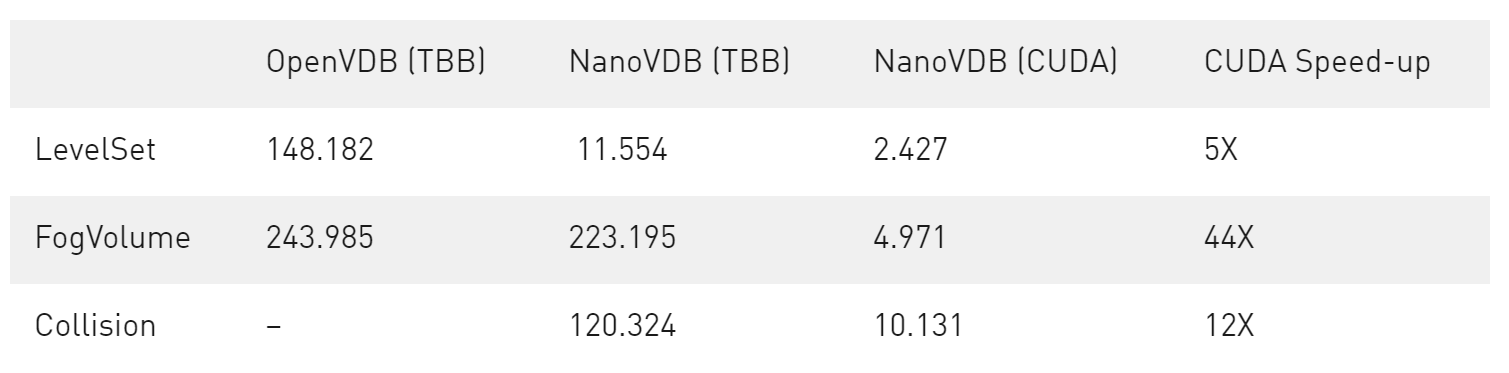
\includegraphics[width=0.75\textwidth]{res/nvidia_benchmark.png}
	\caption{Benchmark results published by NVIDIA. The benchmark setup and source code are undisclosed. \cite{nanovdb_nvidia}}
	\label{fig::nvidia_benchmark}
\end{figure}

For the process simulations the results for level-set raytracing are of significant importance. 
According to Fig. \ref{fig::nvidia_benchmark} NanoVDB on a GPU should be 60x faster compared to a multithreaded implementation using OpenVDB. (Execution time of 2.427ms vs 148.182ms).

However since the benchmark setup and source code are no published it is not clear if the same increase in performance can be achieved for other applications.
Therefore the goal of this paper is to verify these results using a benchmark that is tailored to typical applications within the semiconductor process simulation.

